\chapter{Pharmacometrics}

Pharmacokinetics (PK) is the study of how the body processes a drug. The overall process, from drug administration to drug elimination, can be divided into four phases: absorption, distribution, metabolism, and excretion. These four phases, elaborated in Section \ref{Sec: ADME and PK-parameters}, are often referred to by their acronym ADME. The overall PK process is typically modeled by the aid of compartment models, elaborated in Section \ref{sec: compartment models}, accompanied by a number of PK parameters with a clear physiological interpretation in relation to drug absorption, distribution and elimination. 

Pharmacodynamics (PD), elaborated in Section \ref{sec: Pharmacodynamics}, is the study of the effects of a drug on the body.  In Section \ref{sec: PK/PD-modelling} a PK/PD approach to model delayed effect is introduced.

\section{Pharmacokinetics: ADME} \label{Sec: ADME and PK-parameters}

% \subsection*{Absorption}
The \textbf{absorption} phase describes the process of the drug being absorbed into the systemic circulation after drug administration. The three main routes of drug administration are orally, i.e. by tablet, subcutaneous (SQ), i.e. by injection, or intravascular (IV), i.e. directly into vein. The drug absorption process is typically described through the absorption rate parameter $k_a$ ([1/hour]).

Another important parameter in relation to drug absorption is the bioavailability, $F \in [0,1]$, which denotes the fraction of the administered drug dose, that reaches the systemic circulation. The mass of drug delivered to the systemic circulation is then the product of the given dose, $D$, and $F$, i.e. $F \cdot D$.

Drugs administered IV require no absorption phase as the drug is delivered directly into the systemic circulation, with a bioavailability of $F=1$. Drugs administered extravascularly (EV), i.e. not injected directly into the systemic circulation, require an absorption phase, resulting in a bioavailability of $F <1$.

% \subsection*{Distribution}
The \textbf{distribution} of drug into various tissues of the body (e.g. fat, muscle, and brain tissue) occurs when the drug is absorbed into the systemic circulation. The distribution of drug is modelled in a compartment model setup with exchange rate parameters describing the exchange of drug between compartments. In two-compartment models (introduced in Section \ref{sec: compartment models}), the exchange rate parameters are $k_{12}$ and $k_{21}$ ([1/hour]), which represent the rates of drug exchange between the central and peripheral compartments, respectively. 

The distribution of a drug depends on its biochemical properties as well as the physiology of the individual taking it. In this phase, the drug reaches its place of action and the aim is to achieve the desired drug concentration. 

Drug concentration is measured as the concentration of drug in the plasma, $C$ ([mg/L]), regardless of the place of action of the drug. The primary parameter describing drug distribution is the volume of distribution, $V$ ([L]), that is the total volume a drug has to distribute uniformly into to reach a given concentration in the plasma. Drugs with larger $V$ are thereby exchanged more to other tissues than drugs with lower $V$. The relation between the concentration of drug in the plasma and the volume of distribution is
\begin{align} \label{eq: Concentration}
    C = \frac{A}{V},
\end{align}
where $A$ ([mg]) is the amount of drug. 


% \subsection*{Metabolism}
The \textbf{metabolism} phase, reached after the drug has been absorbed and distributed throughout the body, refers to the process in which the body chemically alters the molecules of a drug, which creates new compounds called metabolites. 
The majority of metabolism occurs in the liver, but it can occur in many areas of the body  including the gastrointestinal tract, kidneys, and plasma.

The metabolism is a part of the elimination of the drug, i.e. the process of removing the administered drug from the body. Any drug that is not eliminated from the body through metabolism is instead eliminated by excretion.


% \subsection*{Excretion}
Drug \textbf{excretion} is the removal of the administered drug and its metabolites from the body. Drugs can be excreted by several routes including the liver, lungs, gastrointestinal tract, and skin, however most drugs are excreted through the kidneys with urine. 

The primary PK parameter describing the elimination of the drug through metabolism and excretion is clearance, $CL$ ([L/hour]), which states the volume of plasma cleared of drug within a certain time interval, thereby representing the efficiency of drug elimination. 

The first order elimination rate constant, $k_e$ ([1/hour]), is defined by the clearance and volume of distribution as 
\begin{align} \label{eq: elimination rate constant}
    k_e = \frac{CL}{V}.
\end{align}
That is, $k_e$ is the fraction of volume cleaned in a certain time interval, typically per hour.


\section{Compartment Models} \label{sec: compartment models}

Compartment models are a central tool in describing the overall drug processing in the body. They consist of a central compartment, zero or more peripheral compartments, and, if the route of administration is EV, a depot (absorption site). The central compartment represents the plasma and highly perfused tissues (such as lungs, liver and kidneys), where drug concentration is measured. If the drug cannot be reasonably assumed to distribute instantly and homogeneously through the entire system after absorption, peripheral compartments can be included to represent poorly perfused tissues (such as muscle and skin), where the drug distributes to and from the central compartment. 

% Peripheral compartments can be included if the drug cannot be reasonably assumed to distribute instantly and homogeneously through the entire system after absorption.

% In Figure \ref{fig: One-compartment model}, a one-compartment model with depot is schematically depicted. In a one-compartment model, the body is be represented as a single compartment in which the distribution of the drug is instantaneous and homogeneous through the entire system after absorption. This is, however, often an extreme simplification in practice \citep[p. 174]{Talevi2024}.

% In Figure \ref{fig: Two-compartment model}, a two-compartment model without depot is schematically depicted. In a two-compartment model, the body is represented with a central compartment consisting of the plasma and highly perfused tissues (such as lungs, liver and kidneys), and a peripheral compartment representing poorly perfused tissues (such as muscle and skin). In the two-compartment model, the drug is thereby not assumed to be evenly distributed throughout the body, but instead distributed between these two different compartments. This is the idea of compartmental modeling with two or more compartments; grouping together tissues with similar blood flow rates to allow for the parameters to be more accurately estimated \citep{chen2024pharmacokinetics}.

% ASSUMPTIONS ON THE MODEL %
The one-compartment model only contains a central compartment, while the two-compartment model also contains a peripheral compartment.
In both models, elimination only occurs from the central compartment and follows first order kinetics, meaning the rate of elimination is proportional to the amount of drug left in the central compartment. With EV administration, a depot is included in the model, and absorption into the central compartment follows first order kinetics, meaning that the rate of absorption is proportional to the amount of drug left in the depot. 
In the two-compartment model, the drug initially enters the central compartment. Furthermore, the distribution of drug from the central compartment to the peripheral compartment, and vice versa, follows first order kinetics. 

% WHAT TO SPECIFY 
Many scenarios can be represented using compartmental modeling, provided that the following are specified: 1) number of compartments (one, two, or more), 2) route of administration (IV, oral, SQ, etc.), implying whether a depot is included or not, and 3) dosage regimen (single/multiple dosage (see Appendix \ref{app: other dosage regimen}) etc.).


% MODELS IN THIS REPORT 
The models of consideration are the one-compartment model with and without depot, and the two-compartment model with depot, all with dosage regimen being a single dose. The compartment model structure is formalised by deriving expressions for the amount of drug in the central compartment as a function of time using ordinary differential equations (ODEs). 


% Drug absorption either follows zero order kinetics (meaning the rate of absorption is constant, e.g. constant rate IV infusion) or first order kinetics (e.g. oral administration).


% Many different scenarios can be modelled using compartment models. To construct the correct model for a given scenario, one should always specify
% \begin{enumerate}[label=\arabic*)]
%     \item assumed number of compartments (one, two, or more), \label{item: ass number of comp}
%     \item route of administration (IV, oral, SQ, etc.), and \label{item: route of adm}
%     \item dosage regimen (single dosage, constant rate infusion, multiple dosage, etc.).
% \end{enumerate}
\begin{figure}[h]
    \centering
    \begin{subfigure}[b]{0.48\textwidth}
    \centering
        \begin{tikzpicture}[node distance=1cm, >=Stealth, thick, scale=1, transform shape] % Smaller figure
      % Absorption Model
      \node[draw, fill=white!10, minimum width=2.5cm, minimum height=1.2cm, align=center] (absorption) {Depot};
      \node[draw, fill=gray!10, minimum width=2.5cm, minimum height=1.2cm, right=1.5cm of absorption, align=center] (central) {Central};

      % Arrows for Absorption Model
      \node[above=0.6cm of absorption] (labelFA) {$\ F \cdot D$}; % Moved label higher
     \draw[<-] (absorption.north) ++(0,-0.36) -- ++(0,1);
      \draw[->] (absorption.east) -- (central.west) node[midway, above] {$k_a$};
      \draw[->] (central.south) -- ++(0,-1) node[midway, right] {$k_e$};
    \end{tikzpicture}
        \caption{One-compartment model with depot (EV administration).}
        \label{fig: One-compartment model}
    \end{subfigure}
    \hfill
    \begin{subfigure}[b]{0.48\textwidth}
        \centering
\begin{tikzpicture}[node distance=1cm, >=Stealth, thick, scale=1, transform shape] 
    % Two-Compartment Model
    \node[draw, fill=gray!10, minimum width=2.5cm, minimum height=1.2cm, align=center] (central2) {Central};
    \node[above=0.6cm of central2] (labelA0) {$D$}; % Moved label higher
     \draw[<-] (central2.north) ++(0,-0.36) -- ++(0,1);
    \node[draw, fill=gray!10, minimum width=2.5cm, minimum height=1.2cm, right=1.5cm of central2, align=center] (peripheral) {Peripheral};

    % First Arrow (top)
    \draw[->] (central2.east) ++(0,0.1) -- ++(1.5,0) node[midway, above] {$k_{12}$};
    
    % Second Arrow (bottom) with vertical shift
    \draw[<-] (central2.east) ++(0, -0.1) -- ++(1.5,0) node[midway, below] {$k_{21}$};
    
    % Vertical Arrow
    \draw[->] (central2.south) -- ++(0,-1) node[midway, right] {$k_e$};
\end{tikzpicture}
        \caption{Two-compartment model without depot (IV administration).}
        \label{fig: Two-compartment model}
    \end{subfigure}
    \caption{Compartment models illustrating drug movement in the body. The grey boxes represent compartments; each representing a homogeneous system in which the drug is assumed to be uniformly distributed. The white box illustrates a depot that drugs administrated EV have to pass through to reach the systemic circulation. The arrows from $F \cdot D$ and $D$ indicate the amount of drug that reaches systemic circulation, while the arrows between the compartments represent drug transitions. The transitions are described by the rate constants $k_a, k_e, k_{12}$ and $k_{21}$.}
    \label{fig: Compartment models}
\end{figure}

\subsection{One-compartment model}
The one-compartment model is depicted in Figure \ref{fig: One-compartment model} without the depot. The mass balance equation for the central compartment is given by the ODE
\begin{align} \label{eq: first order kinetic of amount in one com without abs}
    \Dif{A_{c}(t)} = - k_e * A_{c}(t),
\end{align}
where $A_{c}(t)$ is the amount of drug in the central compartment at time $t$. The solution to \eqref{eq: first order kinetic of amount in one com without abs} is given by
\begin{align} \label{eq: sol to first order kinetic of amount in one com without abs}
    A_{c}(t) = D * \exp(-k_e * t). 
\end{align} 

\subsection{One-compartment model with depot}
The one-compartment model with depot is depicted in Figure \ref{fig: One-compartment model}. The mass balance equation for the central compartment is given by the system of two ODEs
\begin{align} \label{eq: first order kinetic of amount in central com with abs com}
    \Dif{A_{d}(t)}    &= - k_a * A_{d}(t) \nonumber\\
    \Dif{A_{c}(t)} &= k_a * A_{d}(t) - k_{e} * A_{c}(t),
\end{align}
where $A_{d}(t)$ is the amount of drug in the depot at time $t$.
% The first term on the right hand side represents the rate of drug absorbed by the central compartment, while the last term represents the rate of drug eliminated from the central compartment.
The solution to \eqref{eq: first order kinetic of amount in central com with abs com} is given by
\begin{align} \label{eq: sol to first order kinetic of amount in central com with abs com}
    A_{c}(t) = \frac{k_a F D}{k_a - k_e} \left( \exp(-k_e * t) - \exp(-k_a * t) \right).
\end{align}

\subsection{Two-compartment model with depot}
The two-compartment model with depot is depicted in Figure \ref{fig: Two-compartment model} with an added depot. The mass balance equations for the central and peripheral compartments are given by the system of three ODEs
\begin{align}
    \Dif{A_{d}(t)}    &= - k_a * A_{d}(t) \nonumber \\
    \Dif{A_{c}(t)}    &= k_a * A_{d}(t) + k_{21} * A_{p}(t) - k_{12} * A_{c}(t) - k_e * A_{c}(t), \label{eq: 2-comp central}\\
    \Dif{A_{p}(t)} &= k_{12} * A_{c}(t) - k_{21} * A_{p}(t),\nonumber
\end{align}
% \begin{align*}
%     \Dif{A_{c}(t)}    &= k_{21} * A_{p}(t) - k_{12} * A_{c}(t) - k_e * A_{c}(t),\\
%     \Dif{A_{p}(t)} &= k_{12} * A_{c}(t) - k_{21} * A_{p}(t),
% \end{align*}
where $A_p(t)$ is the amount of drug in the peripheral compartment at time $t$. The solution to \eqref{eq: 2-comp central} is given by
\begin{align*}
    A_{c}(t) = D  k_{a} \left( \frac{A e^{-\alpha t} \left( e^{(\alpha - k_{a})t} - 1 \right)}{\alpha - k_{a}} + \frac{B e^{-\beta t} \left( e^{(\beta - k_{a})t} - 1 \right)}{\beta - k_{a}} \right),
\end{align*}
where $A = \frac{\alpha - k_{21}}{\alpha - \beta}$, $B = \frac{k_{21} - \beta}{\alpha - \beta}$, $\alpha + \beta = k_{12} + k_{21} + k_{e}$ and $\alpha \beta = k_{21} * k_{e}$.


% \begin{align*}
%     A_{c}(t) = \psi * \exp(- \alpha t) + \gamma * \exp(- \beta t),
% \end{align*}
% where $\psi = \frac{D * (\alpha - K_{21})}{\alpha - \beta}$, $\gamma = \frac{D * (k_{21} - \beta)}{\alpha - \beta}$, $\alpha + \beta = k_{12} + k_{21} + k_{e}$ and $\alpha \beta = k_{21} * k_{e}$.


% \subsection{Formalizing Compartment Dynamics: Multiple scenarios}



% Consider the scenario of a one-compartment model with IV administration of a single dose $D$. This is equivalent with the model shown in Figure \ref{fig: One-compartment model}, without the absorption site, meaning that $D$ is injected directly to the central compartment. Assuming drug elimination follows first order kinetics, the rate of change in the central compartment, also known as the mass balance equation for the central compartment, is given by the differential equation
% \begin{align} \label{eq: first order kinetic of amount in one com without abs}
%     \Dif{A_{central}(t)} = - k_e * A_{central}(t),
% \end{align}
% where $A_{central}(t)$ denotes the amount of drug in the central compartment at time $t$, and $k_e$ denotes the elimination rate constant. The solution to \eqref{eq: first order kinetic of amount in one com without abs} is given by
% \begin{align} \label{eq: sol to first order kinetic of amount in one com without abs}
%     A_{central}(t) = D * \exp(-k_e * t). 
% \end{align} 

% Consider the scenario of a one-compartment model with EV administration of a single dose $D$, represented in Figure \ref{fig: One-compartment model}. Assuming drug absorption and elimination follows first order kinetics, the mass balance equation for the central compartment is given by 
% \begin{align} \label{eq: first order kinetic of amount in central com with abs com}
%     \Dif{A_{central}(t)} = K_a * A_{absorption}(t) - K_{e} * A_{central}(t),
% \end{align}
% where $A_{absorption}$ denotes the amount of drug at the absorption site and $K_a$ is the absorption rate constant. The first term on the right hand site represents the rate of drug absorbed by the central compartment, while the last term represents the rate of drug eliminated from the central compartment.
% The solution to \eqref{eq: first order kinetic of amount in central com with abs com} is given by
% \begin{align} \label{eq: sol to first order kinetic of amount in central com with abs com}
%     A_{central}(t) = \frac{K_a F D}{K_a - k_e} \left( \exp(-k_e * t) - \exp(-K_a * t) \right).
% \end{align}

% In some cases, a one-compartment model might be a too restrictive assumption. Therefore, consider a two-compartment model with IV administration of a single dose, represented in Figure \ref{fig: Two-compartment model}. Assuming the drug absorption, elimination, and distribution between the compartments follow first order kinetics, the mass balance equations for the two compartments constitute a system of two differential equations given by
% \begin{align*}
%     \Dif{A_{central}(t)}    &= K_{21} * A_{peripheral}(t) - K_{12} * A_{central}(t) - k_e * A_{central}(t),\\
%     \Dif{A_{peripheral}(t)} &= K_{12} * A_{central}(t) - K_{21} * A_{peripheral}(t),
% \end{align*}
% where $A_{peripheral}(t)$ denotes the amount of drug in the peripheral compartment, $K_{21}$ denotes the rate constant representing the flow of drug from the peripheral compartment to the central compartment, and $K_{12}$ denotes the rate constant representing the flow of drug from the central compartment to the peripheral compartment.
% Since the concentration of drug is measured in the plasma, only the solution for the central compartment is necessary. The solution is given by
% \begin{align*}
%     A_{central}(t) = \psi * \exp(- \alpha t) + \gamma * \exp(- \beta t),
% \end{align*}
% where $\psi = \frac{D * (\alpha - K_{21})}{\alpha - \beta}$, $\gamma = \frac{D * (K_{21} - \beta)}{\alpha - \beta}$, $\alpha + \beta = K_{12} + K_{21} + K_{e}$ and $\alpha \beta = K_{21} * K_{e}$.

% It is possible to consider other dosing regimens and more complex compartment structures to obtain more realistic models. Accurate models are, of course, desirable, but a simple one- or two-compartment model might be sufficient enough to obtain an acceptable PK profile, i.e. estimates of the PK parameters listed in Table \ref{tab: pharmacokinetic parameters summary}, of a drug.

% In practice, it is the concentration of the drug in the plasma, $C(t)$, that is measured. For this reason, it is necessary to represent the solutions in terms of concentration which is related to $A(t)$ by \eqref{eq: Concentration}.


\section{Pharmacodynamics} \label{sec: Pharmacodynamics}
The objective of pharmacodynamics (PD) is to model the effect of a drug. For a drug to produce an effect, the drug molecule has to interact with cells. The interaction occurs as a drug molecule attaches to a receptor. Each cell membrane is covered with receptors, where drug molecules can bind. Once a drug molecule binds to a receptor, that receptor becomes blocked, preventing other drug molecules from binding to it. The process of interaction can be described as
\begin{align} \label{eq: Reversible receptor}
    [M] + [R] & \overset{k_1}{\underset{k_{-1}}{\rightleftarrows}} [MR],
\end{align}
where, $[M]$ is the amount of unbounded drug molecules, $[R]$ is the unoccupied receptors, and $[MR]$ is the bound drug/receptor complex, being the association that occurs when a drug molecule binds to a receptor. The constant $k_1$ indicates the rate at which unbound receptors become occupied, and $k_{-1}$ represents the rate at which bound receptors revert to be unbounded. The relation $K_d = k_{-1}/k_1$ is the disassociation.
The rate of change in amount of bound receptor complexes is expressed as
\begin{align} \label{eq: steady state PD}
    \Dif{[MR]} = k_1 [R][M] - k_{-1}[MR],
\end{align}
where on the right hand side, the first term is the rate at which molecules bind to receptors, and the second term is the rate at which the receptors revert to be unbounded. 
The effect of a drug is quantified as 
\begin{align} 
    E &= \varphi[MR] \label{eq: effect formalisation}
\end{align}
as only a proportion, $\varphi \in [0, 1]$, of the complexes are active, i.e. yield an effect.
The maximal effect, $E_{max}$, is achieved when the total number of receptors, $[R_{tot}] = [R] + [MR]$, are occupied. Hence,
\begin{align}
    E_{\text{max}} = \varphi[R_{tot}]. \label{eq: effect formalisation2}
\end{align}

The PD parameters of interest are $E_{max}$ and $K_d$, hence the effect is rewritten as 
\begin{align}
    E = \frac{E_{\text{max}}[M]}{[M] + K_d}, \label{eq: effect with m and kd}
\end{align}
derived from \eqref{eq: steady state PD}, \eqref{eq: effect formalisation}, \eqref{eq: effect formalisation2}, and the expression for $R_{tot}$, see Appendix \ref{app: }.
The parameters are estimated using the Sigmoid $E_{\text{max}}$ model,
\begin{align}\label{eq: sigmoid emax}
    E(C) = E_0 + \frac{E_{\text{max}}C^n}{C^n+C_{50}^n}, 
\end{align}
which approximates \eqref{eq: effect with m and kd} with $C$ representing $[M]$ and $C_{50}$ representing $K_d$, while allowing a baseline effect, $E_0$. By definition, $C_{50}$ is the concentration at which the effect reaches $50\%$ of its maximal increase from baseline, i.e. $E(C_{50}) = E_0 + 1/2 E_{\text{max}}$. The parameter $n$ provides a further degree of flexibility.

\begin{figure}[H]
    \centering
    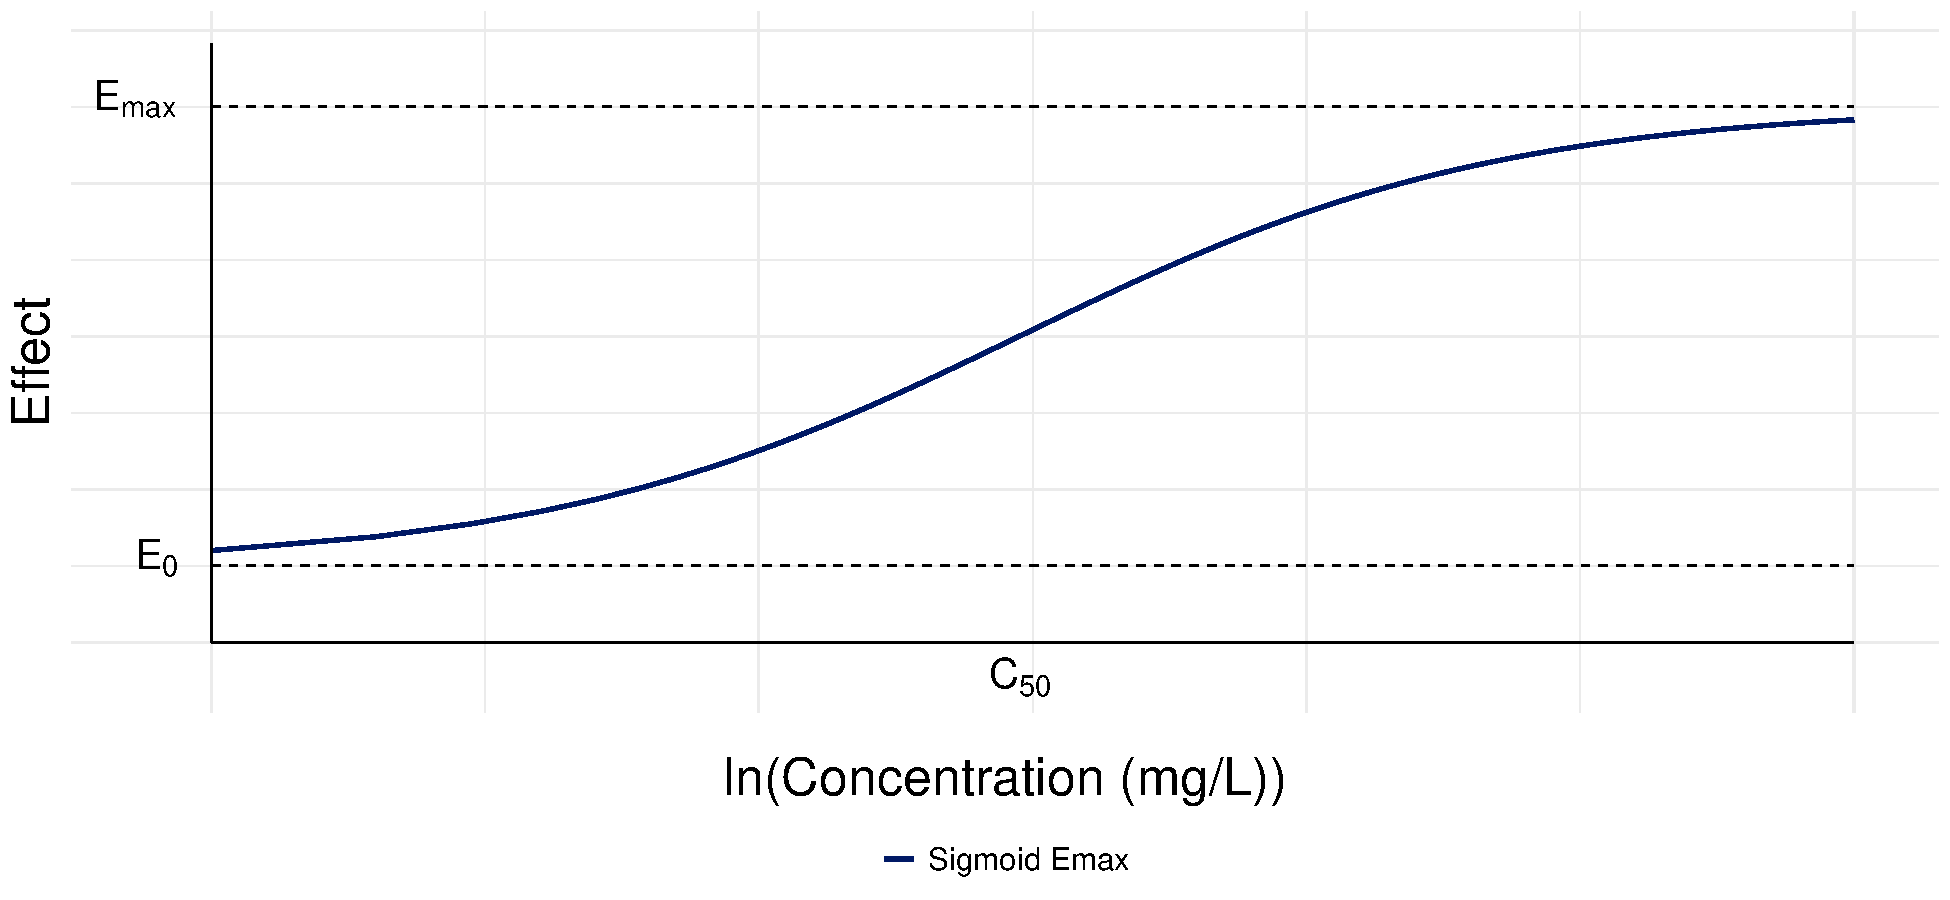
\includegraphics[width=0.9\linewidth]{fig/img/PD/ModelPlots.pdf}
    \caption{Example of $\ln(\text{Concentration})$ vs. PD-models.}
    \label{fig: Different PD-models}
\end{figure}

The effect may be delayed relative to the concentration level. The delay in effect can be modeled by including a hypothetical effect compartment, into the compartmental model used in PK. The effect compartment distributes a negligible amount of concentration from and to the central compartment, see Figure \ref{fig: One-compartment model with effect}, thus having no impact on the concentration within the central compartment.
\begin{figure}[H]
    \centering
    \begin{tikzpicture}[node distance=1cm, >=Stealth, thick, scale=1, transform shape] % Smaller figure
      % Absorption Model
      \node[draw, fill=white!10, minimum width=2.5cm, minimum height=1.2cm, align=center] (absorption) {Absorption};
      \node[draw, fill=gray!10, minimum width=2.5cm, minimum height=1.2cm, right=1.5cm of absorption, align=center] (central) {Central};
      \node[draw, fill=gray!15, minimum width=2.5cm, minimum height=1.2cm, above=1.5cm of central, align=center] (effect) {Effect};

      % Arrows for Absorption Model
      \node[above=0.6cm of absorption] (labelFA) {$\ F \cdot D$}; % Moved label higher
    \draw[<-] (absorption.north) ++(0,-0.36) -- ++(0,1);
    \draw[->] (absorption.east) -- (central.west) node[midway, above] {$k_a$};
    \draw[->] (central.south) -- ++(0,-1) node[midway, right] {$k_e$};

    \draw[dotted, ->] (central.north) ++(0.1,0) -- ++(0,1.5) node[midway, right] {$k_{e1}$};
    
    % Second Arrow (bottom) with vertical shift
    \draw[dotted, <-] (central.north) ++(-0.1, 0) -- ++(0,1.5) node[midway, left] {$k_{e0}$};


    \end{tikzpicture}
    \caption{One compartment model with absorption site and effect compartment.}
    \label{fig: One-compartment model with effect}
\end{figure}
The amount of drug in the effect compartment is described as
\begin{align} \label{eq: Concentration in effect compartment}
    \Dif{A_e} = k_{e1} * A_{\text{central}} - k_{e0} A_e,
\end{align}
where $A_e$ denotes the amount of drug in the effect compartment, $k_{e1}$ denotes the distribution of drug from the central compartment to the effect compartment, $k_{e0}$ denotes the distribution of drug from the effect compartment to the central compartment. The concentration of drug in the effect compartment is defined as
\begin{align*}
    C_e(t) = \frac{k_{e1} D}{V(k_{e1} - k_{e0})} \left( \exp(-k_{e0} * t) - \exp(-k_{e1} * t) \right).
\end{align*}
Drug concentration within the central compartment and effect estimated using the Sigmoid Emax model on the concentration in the effect compartment, is depicted in Figure \ref{fig: PKPDmodel}.
\begin{figure}[H]
    \centering
    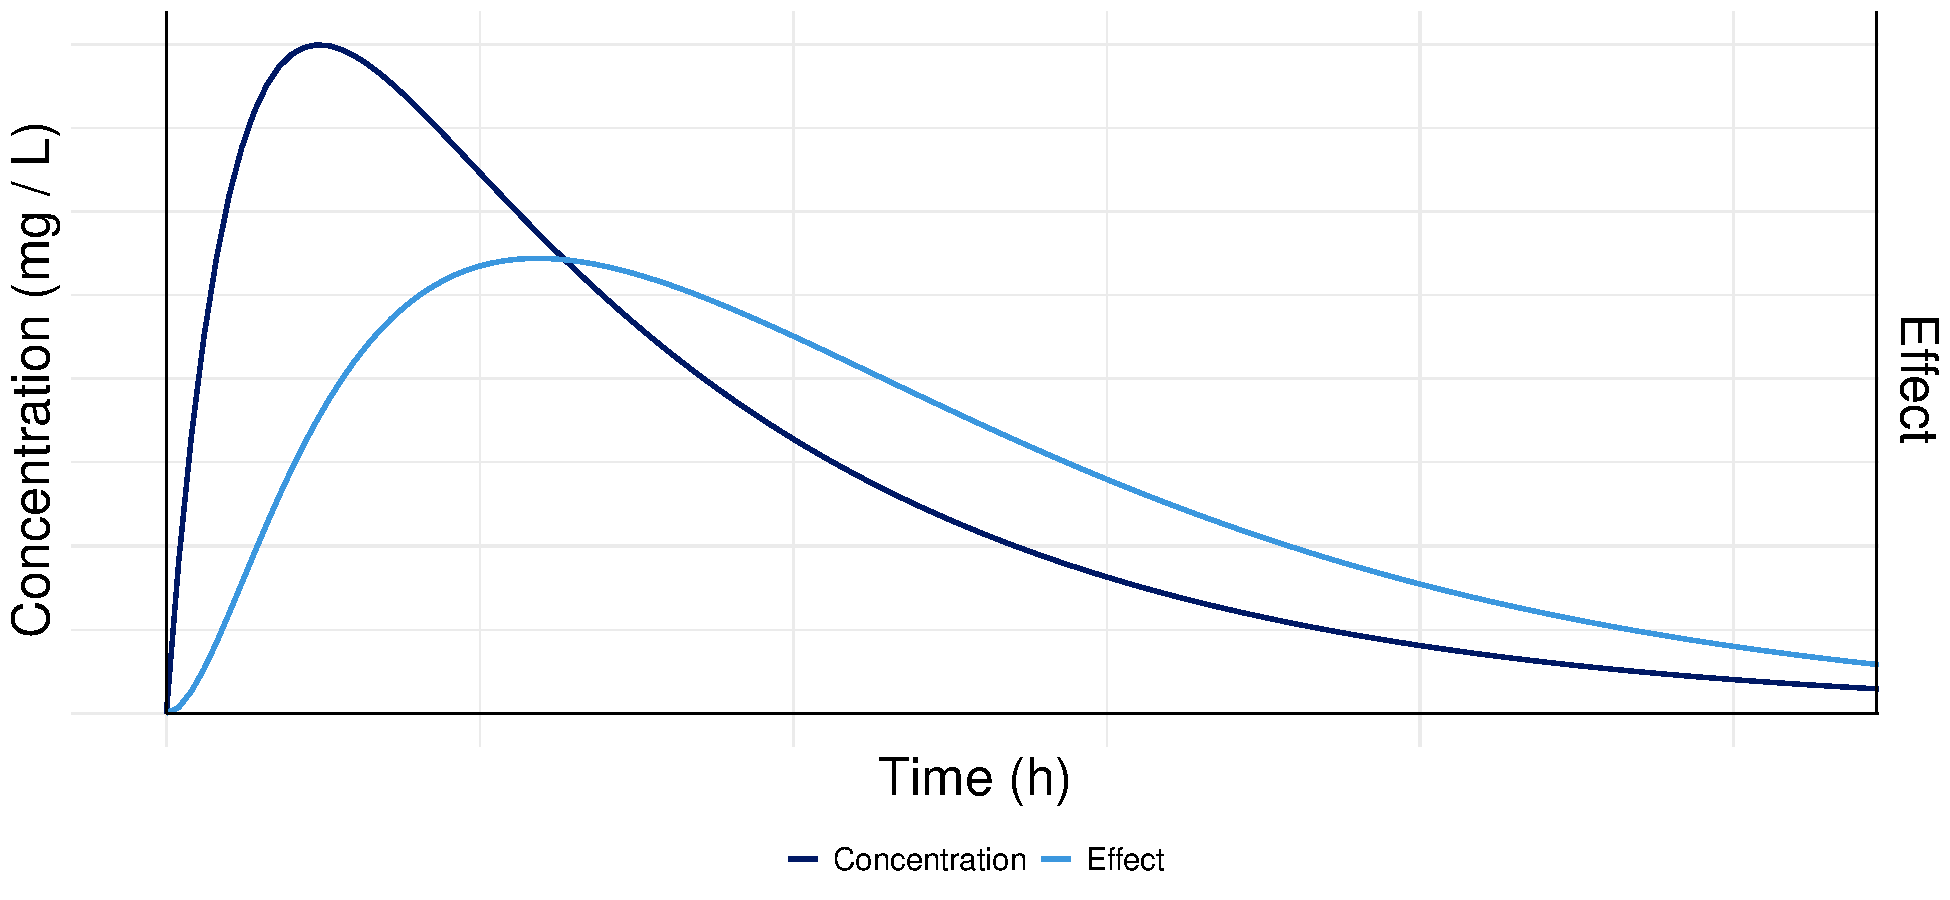
\includegraphics[width=0.95\linewidth]{fig/img/PD/PK-PDmodel.pdf}
    \caption{Concentration and effect relationship of a one-compartment PK model administered EV, incorporating an effect compartment.}
    \label{fig: PKPDmodel}
\end{figure}
Figure \ref{fig: PKPDmodel} shows that the inclusion of an effect compartment in the estimation leads to a delayed effect relative to the concentration levels. \citep{f11a2bf72b3e4305be6ebfffc456fc23}

\section{PK/PD-modelling} \label{sec: PK/PD-modelling}

Sequential PK/PD-modelling is an approach where PK parameters are estimated first using plasma concentration data, and then fixed to fit the PD model.

Simultaneous PK/PD-modelling combines the PK and PD models, and, in addition, allows the effect to be delayed relative to the concentration level measured in the plasma. Given a compartmental PK model, the delay in effect can be modelled by including a hypothetical effect compartment, which distributes a negligible amount of concentration from and to the central compartment, see Figure \ref{fig: One-compartment model with effect}, thus having no impact on the concentration within the central compartment. \begin{figure}[H]
    \centering
    \begin{tikzpicture}[node distance=1cm, >=Stealth, thick, scale=1, transform shape] % Smaller figure
      % Absorption Model
      \node[draw, fill=white!10, minimum width=2.5cm, minimum height=1.2cm, align=center] (absorption) {Depot};
      \node[draw, fill=gray!10, minimum width=2.5cm, minimum height=1.2cm, right=1.5cm of absorption, align=center] (central) {Central};
      \node[draw, fill=gray!15, minimum width=2.5cm, minimum height=1.2cm, above=1.5cm of central, align=center] (effect) {Effect};

      % Arrows for Absorption Model
      \node[above=0.6cm of absorption] (labelFA) {$\ F \cdot D$}; % Moved label higher
    \draw[<-] (absorption.north) ++(0,-0.36) -- ++(0,1);
    \draw[->] (absorption.east) -- (central.west) node[midway, above] {$k_a$};
    \draw[->] (central.south) -- ++(0,-1) node[midway, right] {$k_e$};

    \draw[dotted, ->] (central.north) ++(0.1,0) -- ++(0,1.5) node[midway, right] {$k_{e1}$};
    
    % Second Arrow (bottom) with vertical shift
    \draw[dotted, <-] (central.north) ++(-0.1, 0) -- ++(0,1.5) node[midway, left] {$k_{e0}$};


    \end{tikzpicture}
    \caption{One compartment model with absorption site and effect compartment.}
    \label{fig: One-compartment model with effect}
\end{figure}
The PD model can then be fitted as a sigmoid $E_{\text{max}}$ model with $C=C_e$, the solution to the ODE
\begin{align} \label{eq: Concentration in effect compartment}
    \Dif{C_e}(t) = k_{e1} * C_{\text{c}}(t) - k_{e0} C_e(t),
\end{align}
where $C_e$ and $C_c$ denote the concentration of drug in the effect and central compartment, respectively, and $k_{e1}$ and $k_{e0}$ denote the distribution of drug to and from the effect compartment from and to the central compartment, respectively. 

The simultaneous PK/PD modelling allows for $C_c$ and $C_p$ to be modelled together in a system of ODEs, ensuring that the PK profile dynamically influences the PD response.

Drug concentration within the central compartment and effect estimated using the Sigmoid Emax model on the concentration in the effect compartment, is depicted in Figure \ref{fig: PKPDmodel}.
\begin{figure}[H]
    \centering
    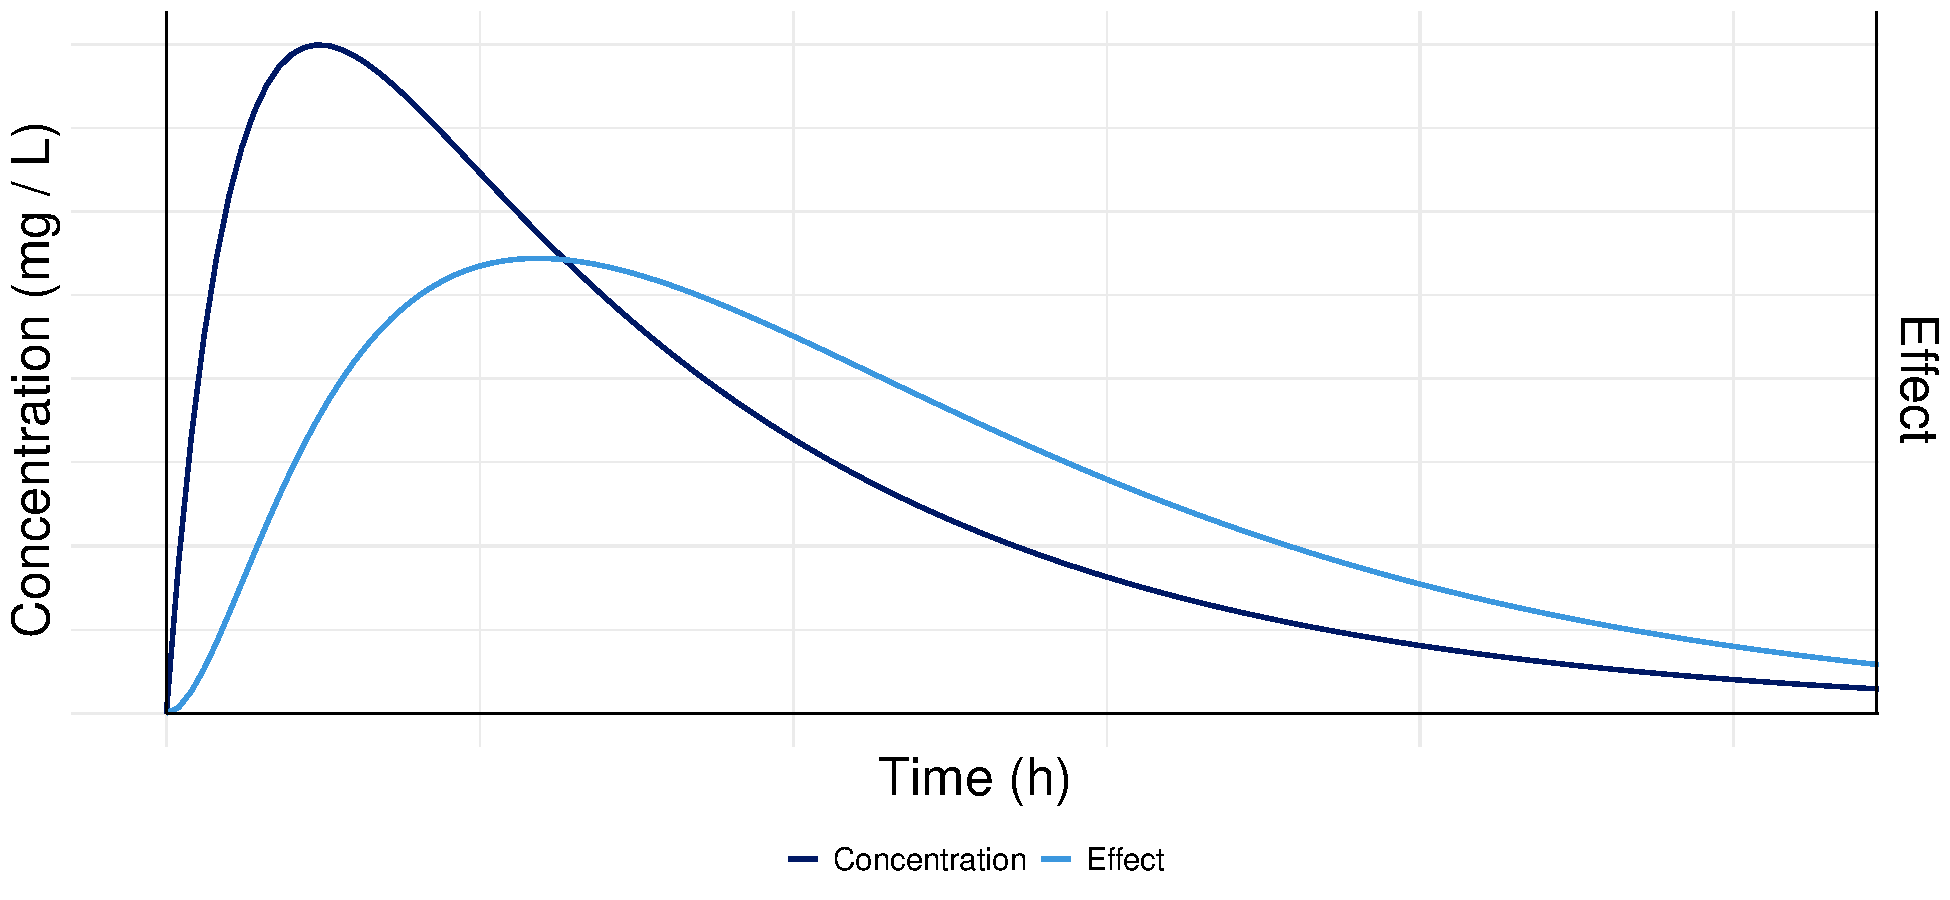
\includegraphics[width=0.95\linewidth]{fig/img/PD/PK-PDmodel.pdf}
    \caption{Concentration and effect relationship of a one-compartment PK model administered EV, incorporating an effect compartment.}
    \label{fig: PKPDmodel}
\end{figure}
Figure \ref{fig: PKPDmodel} shows that the inclusion of an effect compartment in the estimation leads to a delayed effect relative to the concentration levels. \citep{f11a2bf72b3e4305be6ebfffc456fc23}